\documentclass[conference]{IEEEtran}
\IEEEoverridecommandlockouts
% The preceding line is only needed to identify funding in the first footnote. If that is unneeded, please comment it out.
\usepackage{cite}
\usepackage{amsmath,amssymb,amsfonts}
\usepackage{algorithmic}
\usepackage{graphicx}
\usepackage{textcomp}
\usepackage{xcolor}
\usepackage{tabularx}
\usepackage{multirow}
\usepackage{graphics} % for pdf, bitmapped graphics files
\usepackage{subfig}
\usepackage{subcaption}
\usepackage{hyperref}
\usepackage{academicons}
\usepackage{xcolor}
\usepackage{listings}
\usepackage{tabularx} % Asegúrate de incluir este paquete

\usepackage{tikz}
\usetikzlibrary{shapes.geometric, arrows}

\usetikzlibrary{shapes.geometric, arrows}

\tikzstyle{startstop} = [rectangle, rounded corners, minimum width=3cm, minimum height=1cm,text centered, draw=black, fill=red!30]
\tikzstyle{process} = [rectangle, minimum width=3cm, minimum height=1cm, text centered, draw=black, fill=blue!30]
\tikzstyle{arrow} = [thick,->,>=stealth]


\def\BibTeX{{\rm B\kern-.05em{\sc i\kern-.025em b}\kern-.08em
		T\kern-.1667em\lower.7ex\hbox{E}\kern-.125emX}}

% Color Enlace
\definecolor{colorEnlace}{RGB}{0, 0, 0}
\hypersetup{
	colorlinks=true,
	linkcolor=colorEnlace,
	citecolor=colorEnlace,
	urlcolor=colorEnlace,
	pdfauthor={Davis Bremdow Salazar Roa},
	pdftitle={Sistemas Embebidos}
}
\definecolor{mybg}{rgb}{0.97,0.97,0.97}
\definecolor{mygray}{gray}{0.4}
\definecolor{mygreen}{rgb}{0,0.6,0}
\definecolor{myblue}{rgb}{0,0,0.8}
\definecolor{mypurple}{rgb}{0.58,0,0.82}
\definecolor{myred}{rgb}{0.7,0,0}

\lstdefinelanguage{MatlabEnhanced}{
	language=Matlab,
	morekeywords={[2]linspace,plot,title,xlabel,ylabel,legend,grid},
	morekeywords={[3]sin,cos,exp,log,sqrt},
	keywordstyle=\color{myblue}\bfseries,
	keywordstyle=[2]\color{mypurple},
	keywordstyle=[3]\color{myred},
	commentstyle=\color{mygreen}\itshape,
	stringstyle=\color{mygray},
	morecomment=[l]%
}

\lstset{
	language=MatlabEnhanced,
	backgroundcolor=\color{mybg},
	frame=single,
	basicstyle=\ttfamily\small,
	showstringspaces=false,
	numbers=none,              %
	xleftmargin=0pt,           %
	framexleftmargin=0pt,      
	framexrightmargin=0pt,
	framextopmargin=2pt,
	framexbottommargin=2pt,
	breaklines=true,
	tabsize=1,
}

% Control 
\usepackage{amsmath}
\begin{document}
	
	\title{Análisis de Ruido en una señal FM}
	\author{
		\makebox[\textwidth][c]{\large\textbf{Universidad Nacional de San Antonio Abad del Cusco}}\\
		\makebox[\textwidth][c]{\normalsize\textit{Escuela profesional de Ingeniería Electrónica}}\\
		\makebox[\textwidth][c]{\normalsize\textit{Telecomunicaciones I}}\\
		\and
		\IEEEauthorblockN{Ing. Milton Velasquez Curo}
		\IEEEauthorblockA{Ingeniero Electrónico \\
			Cusco, Perú \\
			milton.velasquez@unsaac.edu.pe}
		\and
		\IEEEauthorblockN{Ruth Juana Espino Puma - 185746}
		\IEEEauthorblockA{Estudiante de Ingeniería Electrónica \\
			Cusco, Perú \\
			184657@unsaac.edu.pe}
		\and
		\IEEEauthorblockN{Davis Bremdow Salazar Roa - 200353}
		\IEEEauthorblockA{Estudiante de Ingeniería Electrónica \\
			Cusco, Perú \\
			200353@unsaac.edu.pe}
	}
	
	\maketitle
	\begin{abstract}
		
	\end{abstract}
	
	\begin{IEEEkeywords}
		Modulación FM, SNR
	\end{IEEEkeywords}
	
	%% Contenido del documento
	\section{ SNR en la demodulación FM}
	
	La SNR en FM se define como la relación entre la potencia media de la señal modulada y la potencia media del ruido en una portadora sin modular, implicando que el ruido en la señal moduladora no influye significativamente en este tipo de esquema.
	
	
	
	\section{ Metodología }
	Para poder cuantizar la influencia del generador de ruido en la demodulación FM, es de vital importancia poder modificar los parámetros de una señal FM, siendo que dentro de ello se debe considerar, el ancho de banda de la señal de información, la desviación máxima estándar y en función a ello el índice de modulación, además para poder trabajar dentro del ancho de banda de influencia del dispositivo de ruido también fue necesario controlar la frecuencia de transmisión.
	
	En tal sentido para este propósito se definieron 2 proyectos en el software GNU Radio que constituyen a un transmisor y demodulador FM los cuales pudieron facilitar la variación de parámetros.
	
	\section{ Transmisor FM }
	
	En la parte del transmisor FM se definió una modulación WBFM (Wide Band FM) esto con la finalidad de poder modificar el valor de $\beta$ o índice de modulación en el intervalo entre 0 y 10, en la figura \ref{fig:transmisor-fm} se muestra un esquema gráfico para este propósito en el cual para la transmisión se hace uso del bloque WBFM el cual internamente realiza el proceso de mezclado para la generación de una señal FM,, además también se hicieron uso  2
	
	
	\begin{figure}[h]
		\centering
		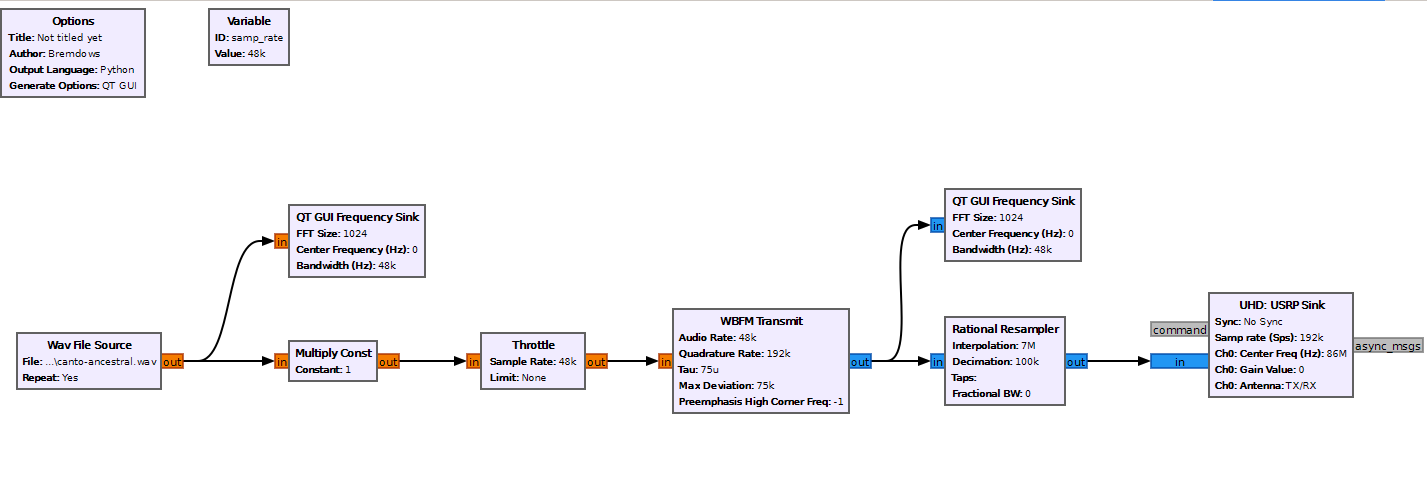
\includegraphics[width=0.5\linewidth]{media/transmisor-fm}
		\caption{SDR: Transmisor FM - GNU Radio}
		\label{fig:transmisor-fm}
	\end{figure}
	
	
	\section{ Receptor FM }
	
	\section{ Análisis de datos }
	
	
	
	
	
	
	\bibliographystyle{IEEEtran}
	\bibliography{biblio}
\end{document}
